\subsection{Part 2: Participation in Consensus}\label{sec:participation}

After a pool is set up, the functionality's second part
(Figure~\ref{fig:Fpool-2}) considers participation in the system, \ie
\emph{validating transactions} and \emph{issuing blocks}.
The pool members continuously monitor the network for new transactions, which
they collect, validate, and organize in a \emph{mempool}.  As mentioned in the
introduction, the pool members \emph{remain online} for the entirety of the
execution to perform the pool's operations. Specifically, when the pool is
elected to participate, the mempool's transactions are serialized and published
in a block. Under PoS, the pool participates proportionally to its
aggregated member and delegated stake.

To improve performance, we define a distributed mechanism for transaction
verification, \ie a \emph{distributed mempool}. Such load balancing mechanism
increases efficiency by requiring only a subset of the pool's members to verify
each transaction. Notably, this is in contrast to the standard practice of
Bitcoin mining pools, where the pool's operator decides the transactions to be
mined by its members; instead, our approach further reduces these trust
requirements.

To construct a distributed mempool, we consider a subselection mechanism to
identify the parties that verify each transaction. This mechanism should be:
\begin{inparaenum}[a)]
    \item \emph{non-interactive}
    \item \emph{deterministic},
    \item \emph{balanced}, \ie every party should be chosen with the same
        probability.
\end{inparaenum}
Subselection is secure if a majority of the elected committee is honest.
However, since the adversary may corrupt some pool members, this may not always
be the case. We model this uncertainty via the probability
$\prob^{\subselectionParam, \adversarialParties, \totalParties}$, which depends
on the size of the committee and the power of the adversary among the pool's
members.

A straightforward way to implement subselection is to assume that the pool's
members are ordered in a well-defined manner, \eg lexicographically. Given the
ordered list $\partylist = [\p_1, \p_2, \dots, \p_\totalParties]$ of pool
members, we use a permutation algorithm $\permutationAlgo(\cdot, \cdot,
\cdot)$, which takes two arguments,
\begin{inparaenum}[i)]
    \item a transaction $\tx$,
    \item a chain $\chain$, and
    \item the ordered list of pool members $\partylist$,
\end{inparaenum}
and outputs a pseudorandom permuted list $\partylist_{\tx}$. For every
transaction $\tx$ and a given chain $\chain$, the committee responsible for
verification consists of the $\subselectionParam$ first members in
$\partylist_{\tx}$. Naturally, this proposal is rather simple, so alternative,
\eg VRF-based, mechanisms could be proposed to improve performance.

We note that using $\chain$ during the subselection mechanism is important to
avoid adaptive attacks. Specifically, the chain $\chain$ simulates a randomness
beacon, such that at least one of its last $u$ blocks is honest, for some
parameter $u$. If $\chain$ was not used, the adversary could construct a
malicious transaction in such way that the subselected committee would also be
malicious. By using $\chain$ as a seed to the pseudorandom permutation, the
adversary's ability to construct such malicious transaction is limited.
Alternatively, cryptographic sortition~\cite{DBLP:conf/sosp/GiladHMVZ17} could
be employed to fully handle adaptive adversaries.

The (honest) members need to always have the same view of the distributed
mempool; this is achieved via authenticated broadcast. Assuming a Public Key
Infrastracture (PKI), as is our setting, it is possible to achieve deterministic
authenticated broadcast in $t + 1$ rounds for $t$ adversarial
parties~\cite{lamport1982byzantine,pease1980reaching,dolev1983authenticated}.
Each time a party adds a transaction to its mempool, it broadcasts it, such
that, at any point in time, the honest members of the pool have the same view
of the network \wrt the canonical chain and the mempool of unconfirmed
transactions. We remind that, as shown by Garay \etal~\cite{PODC:GKKZ11},
$\Fbroad$ can be implemented to ensure adaptive corruptions using commitments.
We note that, in existing distributed ledgers, the order with which
transactions are added to the mempool does not affect the choice when creating
a new block; for instance, transactions of a new block are typically chosen
based on a fee-per-byte score. If the order of transactions is pertinent, a
stronger primitive like Atomic Broadcast~\cite{defago2004total} could be
employed.

Following, the committee employs a consensus sub-protocol to agree on
the transaction's validity. When a party $\p$ retrieves a new transaction $\tx$
from the network, it broadcasts it as above. Then, each party computes the
permuted list $\partylist_{\tx}$. Each party, which is in the validation
committee for $\tx$, computes locally the validation predicate and submits its
output to the consensus protocol. The consensus protocol should offer
\emph{strong validity}, \ie if all honest parties should have the same input
bit, they should output this bit. Finally, the output of the consensus protocol
is broadcast to the rest of the pool. To verify the committee's actions, a
party may request the transcript of the consensus sub-protocol.

Finally, to compute the probability of electing an honest committee,
we have a hypergeometric distribution, with population size
$\totalParties$ and $\totalParties - \adversarialParties$ honest parties, where
a sample of parties of size $\subselectionParam$ is chosen \emph{without
replacement}. Thus, the probability of honest committee majority is:
$\prob^{\subselectionParam, \adversarialParties, \totalParties} = 1 - \sum_{v = \lfloor \frac{\subselectionParam + 1}{2} \rfloor}^{\min (\subselectionParam, \adversarialParties)} \frac{ {\adversarialParties \choose v} \cdot {{\totalParties - \adversarialParties} \choose {\subselectionParam - v}} }{ {\totalParties \choose \subselectionParam} }.$
Figure~\ref{fig:subselection} provides further intuition on the probability
\wrt the subselection parameter $\subselectionParam$.

\begin{figure}
    \begin{center}
        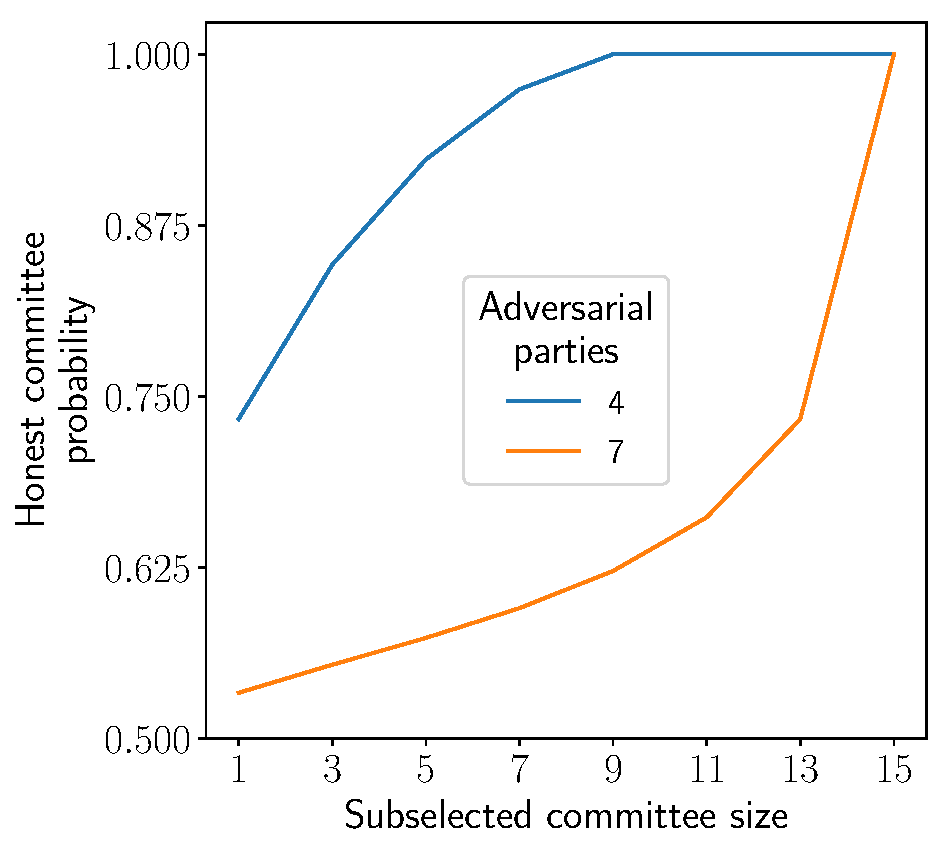
\includegraphics[width=0.5\columnwidth]{figures/collective-pools/probability_subselection.pdf}
    \end{center}
    \caption{
        The probability of subselecting an honest committee \wrt the committee
        size $\subselectionParam$, $\totalParties = 15$ total parties and
        $\lfloor \frac{\totalParties - 1}{3} \rfloor$ and $\lfloor
        \frac{\totalParties - 1}{2} \rfloor$ adversarial parties.
    }
    \label{fig:subselection}
\end{figure}

Following, Figure~\ref{fig:Fpool-2} defines the second part of our
functionality, while Figure~\ref{fig:Ppool-2} presents the second part of our
protocol.

\myhalfbox{Collective Pool Functionality $\Fpool^{\thold,\wfunc}$ (second part)}{white!40}{white!10}{
    \noindent{\bf Transaction Verification:}
        Upon receiving $\msg{transaction}{\tx, \subselectionParam}$ from
        $\p_i$, forward it to $\iadv$. Then send $\mathsf{READ}$ to $\Gledger$
        on behalf of $\p_i$ and wait for the reply $\chain$. Following, set
        $\adversarialParties$ as the number of corrupted parties; with
        probability $\prob^{\subselectionParam, \adversarialParties,
        \totalParties}$ set $b := \algovalidate(\tx, \chain)$, otherwise (with
        probability $1 - \prob^{\subselectionParam, \adversarialParties,
        \totalParties}$), send $\msg{transaction-ver}{\tx}$ to $\iadv$, wait for a reply
        $\msg{transaction-ok}{\chain, \tx, f}$, and set $b := f$. Finally, if
        $b = 1$, insert $\tx$ to $\mathsf{mempool}$ and send
        $\msg{transaction}{\chain, \tx, b}$ to all parties.

    \noindent{\bf Mempool Update:}
        Upon receiving $\msg{transaction}{\chain^\prime, \tx, 1}$ from $\p_i$,
        forward it to $\iadv$. Then send $\mathsf{READ}$ to $\Gledger$ on
        behalf of $\p_i$ and wait for the reply $\chain$. If $\chain^\prime \prec
        \chain$ and $\p_i$ is honest, insert $\tx$ to $\mathsf{mempool}$ and
        return $\msg{mempool-updated}{\tx}$.

    \noindent \noindent{\bf Block issuing:}
        Upon receiving $\msg{issue-block}{}$ from a party $\p$, forward it to
        $\iadv$. When a set of parties $\partyset$ has submitted
        $\msg{issue-block}{}$, if $\sum_{j \in [1, m]} \members[\p_j] >
        \thold$, then for every party $\p_i \in \partyset$, send
        $\mathsf{READ}$ to $\Gledger$ on behalf of $\p_i$ and wait for the
        reply $\chain_i$. If all received chains equal, \ie are the same chain
        $\chain$, remove every $\tx$ in $\mathsf{mempool}$ that also exists in
        $\chain$. Then, set $b = \blockify(\mathsf{mempool})$, send
        $\msg{issue-block}{b}$ to $\iadv$, and wait for the reply
        $\msg{issue-block}{b, \threshsig_{pool}}$.  Following, check if
        $\forall (m, \sigma, b^\prime) \in T: \sigma \neq \threshsig_{pool},
        (b, \threshsig_{pool}, 0) \not \in T$; if the checks hold, insert $(b,
        \threshsig_{pool}, 1)$ to $T$. Finally, reply with $\msg{block}{b,
        \threshsig_{pool}}$.

}{\label{fig:Fpool-2} The second part of the proposed Pool Functionality, which defines the consensus participation operations.}

\myhalfbox{Collective Pool Protocol $\Ppool^{\thold,\wfunc}$ (second part)}{white!40}{white!10}{
    \noindent{\bf Transaction Verification:}
        Upon receiving $\msg{transaction}{\tx, \subselectionParam}$, send
        $\mathsf{READ}$ to $\Gledger$ and wait for the reply $\chain$. Then,
        set $b = \algovalidate(\chain, \tx)$, compute $\partylist^\prime =
        \permutationAlgo(\tx, \chain, \partylist)$ and initiate protocol
        $\Pconsensus$ with the $\subselectionParam$ first parties in
        $\partylist^\prime$ with input $b$. Upon computing the output of
        $\Pconsensus$, $\beta$, send $\msg{transaction}{\chain, \tx, \beta}$ to
        $\Fbroad$ and return it.

    \noindent{\bf Mempool Update:}
        Upon receiving $\msg{transaction}{\chain^\prime, \tx, 1}$, $\p_i$, send
        $\mathsf{READ}$ to $\Gledger$ and wait for the reply $\chain$. If
        $\chain^\prime \prec \chain$, insert $\tx$ to $\mathsf{mempool}$ and return
        $\msg{mempool-updated}{\tx}$.

    \noindent{\bf Block Issuing:}
        Upon receiving $\msg{issue-block}{}$, send $\mathsf{READ}$ to
        $\Gledger$ and wait for the reply $\chain$. For every $\tx$ in
        $\mathsf{mempool}$, if $\tx$ is also in $\chain$, then remove $\tx$
        from $\mathsf{mempool}$. Next, set $b = \blockify(\mathsf{mempool})$
        and send $\msg{Sign}{b}$ to $\Fweight$. Upon receiving a reply
        $\msg{Sign}{b, \threshsig_{pool}}$, return $\msg{block}{b,
        \threshsig_{pool}}$.

}{\label{fig:Ppool-2} The second part of our protocol, which describes the set of operations for consensus participation.}

We note that our design satisfies most of the desiderata outlined in
Section~\ref{sec:collective-pool-desiderata}. Some (\eg pool proportional rewards or stake
reallocation) are dependent on the underlying ledger system's details,
therefore are outside of our scope; nevertheless, our design does not pose
restrictions in capturing them. The reward functionality $\rewardFunc$ handles
the reward-specific desiderata, while $\Fpool$'s first part
(Figure~\ref{fig:Fpool-1}) covers the requirements for permissioned access and
closing of the pool. However, $\Fpool$'s handling of stake reallocation and
updating of the pool's parameters could be more dynamic, as it currently
requires closing and re-creating a pool with the new parameters.
